\documentclass[10pt]{article}
\usepackage[%
left=0.984252in,%
right=0.787402in,%
top=0.787402in,%
bottom=0.787402in,%
paperheight=11in,%
paperwidth=8.5in%
]{geometry}%

\usepackage{xeCJK}
\usepackage{blindtext}
\usepackage[T1]{fontenc}
\usepackage{caption}
\usepackage{graphicx}
\usepackage{textcomp}
\usepackage{fancyhdr}
\usepackage{listings}

\pagestyle{fancy}
\fancyhf{}
\fancyhead[R]{\thepage}
\usepackage{float}
\usepackage{alltt}

\setCJKmainfont{AozoraMinchoRegular.ttf}
\setCJKsansfont{AozoraMincho-bold.ttf}


\setCJKmainfont{AozoraMinchoRegular.ttf}
\setCJKsansfont{AozoraMincho-bold.ttf}

\usepackage{indentfirst}

\title{2 部データ構造とアルゴリズムI レポート課題}
\author{18NC021}
\date{カトリ スザン}
\captionsetup[table]{name=表}
\captionsetup[figure]{name=図}

\begin{document}

\begin{titlepage}
	\maketitle
\end{titlepage}


 
\tableofcontents
\pagebreak


\section{課題1}

\subsection{問題1-1}
\subsubsection{shohin.h}

\begin{lstlisting}[language=C]
    #ifndef C_ALGO_REPORT1_SHOHIN_H
    #define C_ALGO_REPORT1_SHOHIN_H
    
    #endif //C_ALGO_REPORT1_SHOHIN_H
    
    
    #define ZEI (1.08)
    typedef struct{
        char* name;
        int tanka;
        int sotozei;
    } SHOHIN;
    extern SHOHIN shohin[];
    void printshohin(SHOHIN s);
\end{lstlisting}

\subsubsection{shohin.c}

\begin{lstlisting}
    #define N 3
    
    #include <stdio.h>
    #include "shohin.h"
    
    SHOHIN shohin[] = {{"Apple",  150},
                       {"Orange", 100},
                       {"Banana", 200},
                       {"Book1",  500, 1},
                       {"",       0}};
    
    void printshohin(SHOHIN s) {
        printf("%s\t単価%d円(%s)", s.name, s.tanka, s.sotozei ? "外税" : "内税");
    }
\end{lstlisting}

\subsubsection{テストプログラム1-1}
\begin{lstlisting}
    #include <stdio.h>
    #include "shohin.h"
    int main(void){
      int i;
      for(i=0;shohin[i].tanka!=0; i++){
        printf("商品コード %d 品名 ",i);
        printshohin(shohin[i]);
        printf("\n");
      }
      return 0;
    }
\end{lstlisting}


\subsubsection{実行結果}

\begin{figure}[H]
		\centering
		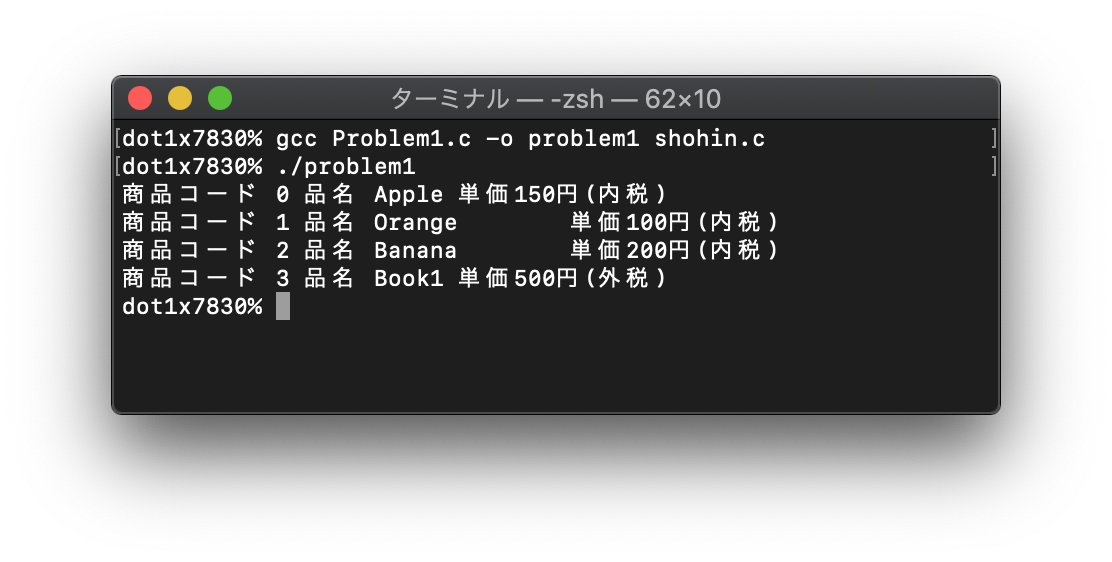
\includegraphics[]{problem1-1.png}
		\caption{問題1-1実行結果}
\end{figure}

\subsubsection{プログラムの解説}
[shohin.c]のprintshohin関数はSHOHIN型のsを引数とし、戻り値はvoidである。
この関数は渡された構造体のname(:string)とtanka(:int)プロパティーをprintする。また最後にstozei(:int)プロパティーの値がtruthy値の場合は'外税'をprintし、falsy値の場合は'内税'をprintする。
\pagebreak


\subsection{問題1-2}
\subsubsection{shohin.h}
    \begin{lstlisting}
    #ifndef C_ALGO_REPORT1_SHOHIN_H
    #define C_ALGO_REPORT1_SHOHIN_H
    
    #endif //C_ALGO_REPORT1_SHOHIN_H
    
    
    #define ZEI (1.08)
    typedef struct{
        char* name;
        int tanka;
        int sotozei;
    } SHOHIN;
    extern SHOHIN shohin[];
    void printshohin(SHOHIN s);
    \end{lstlisting}
\subsubsection{shohin.c}
    \begin{lstlisting}
    #define N 3
    
    #include <stdio.h>
    #include "shohin.h"
    
    SHOHIN shohin[] = {{"Apple",  150},
                       {"Orange", 100},
                       {"Banana", 200},
                       {"Book1",  500, 1},
                       {"",       0}};
    
    void printshohin(SHOHIN s) {
        printf("%s\t単価%d円(%s)", s.name, s.tanka, s.sotozei ? "外税" : "内税");
    }

    \end{lstlisting}
\subsubsection{uriage.h}
    \begin{lstlisting}
    #ifndef C_ALGO_REPORT1_URIAGE_H
    #define C_ALGO_REPORT1_URIAGE_H
    
    #endif //C_ALGO_REPORT1_URIAGE_H
    
    typedef struct {
        int code;
        int num;
    }URIAGE;
    
    int printUriage(URIAGE* q);
    \end{lstlisting}
    \pagebreak
\subsubsection{uriage.c}
    \begin{lstlisting}
    #include <stdio.h>
    #include "uriage.h"
    #include "shohin.h"
    
    int printUriage(URIAGE *q) {
    
        char *const product_name = shohin[q->code].name;
        const int item_price = shohin[q->code].tanka;
        const int tax = shohin[q->code].sotozei;
        const int total_sales = q->num;
        const int total_price =
                tax ? (item_price * total_sales) * ZEI : item_price * total_sales;
        printf("%s\t 単価%d円(%s)\t%d 個\t%d円 \n", product_name, item_price,
               tax ? "外税" : "内税", total_sales, total_price);
        return total_price;
    }
    \end{lstlisting}
\subsubsection{テストプログラム1-2}
    \begin{lstlisting}
    #include <stdio.h>
    #include "shohin.h"
    #include "uriage.h"
    int main(void){
      URIAGE u1={0,3};
      URIAGE u2={3,4};
      int shokei;
      shokei = printUriage(&u1);
      printf("\t%d\n",shokei);
      shokei = printUriage(&u2);
      printf("\t%d\n",shokei);
      return 0;
    }
    \end{lstlisting}
    
\subsubsection{実行結果}
\begin{figure}[H]
	\centering
	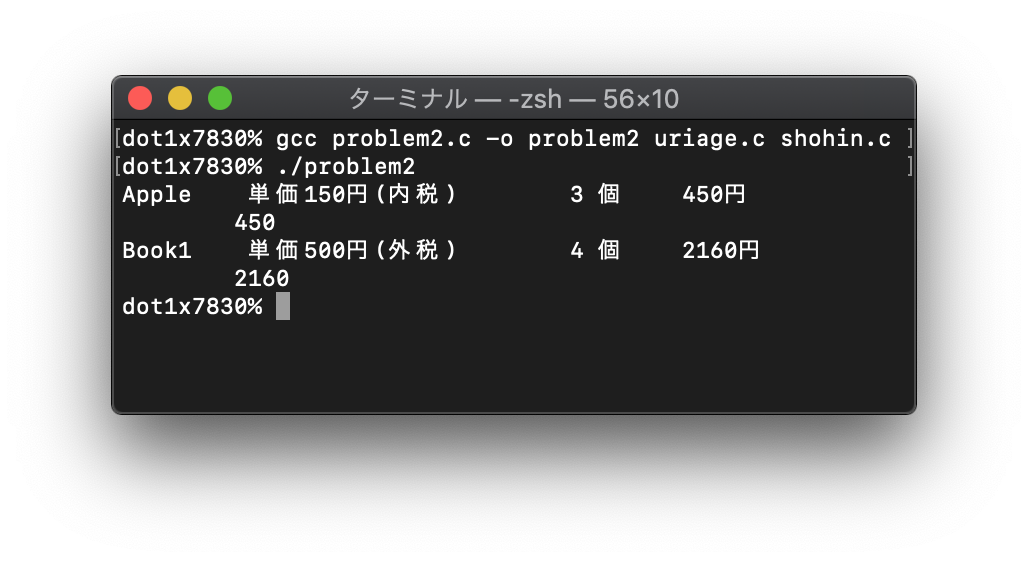
\includegraphics[width=0.7\textwidth]{problem1-2.png}
	\caption{問題1-2実行結果}
\end{figure}

\subsubsection{プログラムの解説}
[uriage.c]のprintUriage関数はURIAGE型のポインター(*q)を引数とし、戻り値がtotal\_price(:int)の関数である。この関数に渡されるポインターにはshohin(:SHOHIN)のインデックスを指定しているcode(:int)プロパティーとそのインデックスの商品の売り上げ数を指定しているnum(:int)プロパティーを持っている構造体のアドレスが格納されている。
この関数は構造体*qで指定されたshohin(:SHOHIN)のあるインデックスに入っている商品の売り上げ総額を計算してtotal\_price(:int)に格納する。そして商品の名前、単価、売り上げ数、売り上げ総額をprintする。最後にtotal\_price(:int)をreturnする。
shohinのsotozeiプロパティーの値がtruthlyの場合は単価に+8\%(税金)を加算して計算する。falsyの場合は税金を加算せずに計算する。また、この関数ではshohinのプロパティーの値を二回以上参照していて、毎回構造体のプロパティーを指定するのが面倒くさい為それぞれのプロパティー用に変数を用意してその値を格納して使っている。
\pagebreak

\subsection{問題1-3}
\subsubsection{shohin.h}
    \begin{lstlisting}
    #ifndef C_ALGO_REPORT1_SHOHIN_H
    #define C_ALGO_REPORT1_SHOHIN_H
    
    #endif //C_ALGO_REPORT1_SHOHIN_H
    
    
    #define ZEI (1.08)
    typedef struct{
        char* name;
        int tanka;
        int sotozei;
    } SHOHIN;
    extern SHOHIN shohin[];
    void printshohin(SHOHIN s);
    \end{lstlisting}
\subsubsection{shohin.c}
    \begin{lstlisting}
    #define N 3
    
    #include <stdio.h>
    #include "shohin.h"
    
    SHOHIN shohin[] = {{"Apple",  150},
                       {"Orange", 100},
                       {"Banana", 200},
                       {"Book1",  500, 1},
                       {"",       0}};
    
    void printshohin(SHOHIN s) {
        printf("%s\t単価%d円(%s)", s.name, s.tanka, s.sotozei ? "外税" : "内税");
    }

    \end{lstlisting}
\subsubsection{uriage.h}
    \begin{lstlisting}
    #ifndef C_ALGO_REPORT1_URIAGE_H
    #define C_ALGO_REPORT1_URIAGE_H
    
    #endif //C_ALGO_REPORT1_URIAGE_H
    
    typedef struct {
        int code;
        int num;
    }URIAGE;
    
    int printUriage(URIAGE* q);
    int printUriageArray(URIAGE u[]);
    \end{lstlisting}
    \pagebreak
\subsubsection{uriage.c}
    \begin{lstlisting}
    #include <stdio.h>
    #include "uriage.h"
    #include "shohin.h"
    
    int printUriage(URIAGE *p) {
        char *const product_name = shohin[p->code].name;
        const int item_price = shohin[p->code].tanka;
        const int tax = shohin[p->code].sotozei;
        const int total_sales = p->num;
        const int total_price =
                tax ? (item_price * total_sales) * ZEI : item_price * total_sales;
        printf("%s\t 単価%d円(%s)\t%d 個\t%d円 \n", product_name, item_price,
               tax ? "外税" : "内税", total_sales, total_price);
        return total_price;
    }
        
    int printUriageArray(URIAGE u[]) {
        int shokei = 0;
        for (int i = 0; u[i].code != -1; i++) {
            shokei += printUriage(&u[i]);
        }
        return shokei;
    }
    \end{lstlisting}
\subsubsection{テストプログラム1-3}
\begin{lstlisting}
    #include <stdio.h>
    #include "shohin.h"
    #include "uriage.h"
    int main(void){
      URIAGE u[]={{0,3},{1,2},{2,1},{3,4},{-1}};
      int shokei;
      shokei = printUriageArray(u);
      printf("\t%d\n",shokei);
      return 0;
    }
\end{lstlisting}
\pagebreak
\subsubsection{実行結果}
 
\begin{figure}[H]
	\centering
	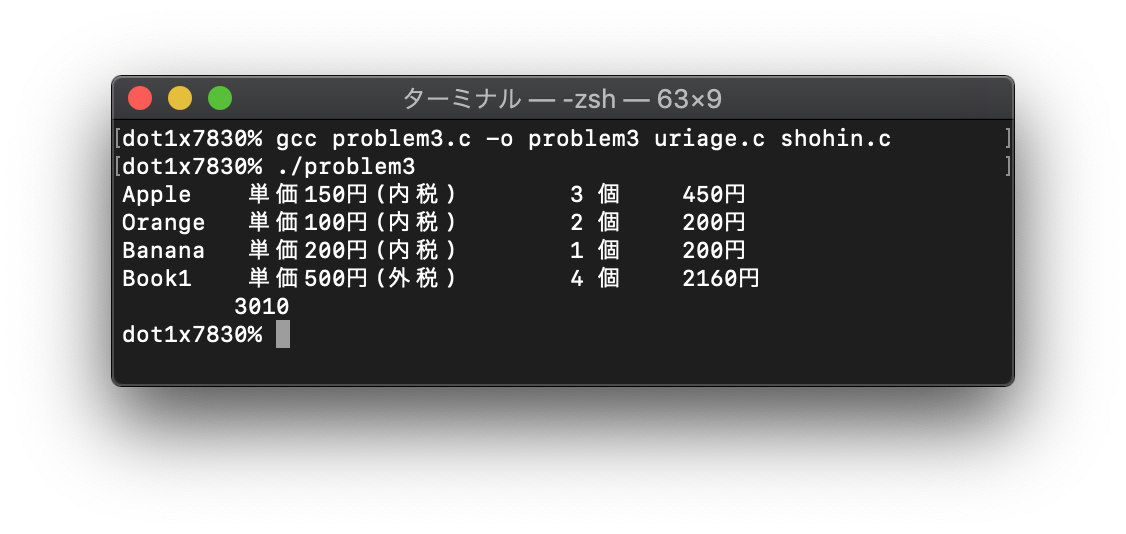
\includegraphics[]{problem1-3.png}
	\caption{問題1-3実行結果}
\end{figure}

\subsubsection{プログラムの解説}
[uriage.c]のprintUriageArray関数はURIAGE型の配列uを引数とし、戻り値がshokei(:int)の関数である。
配列uの各要素にはshohin(:SHOHIN)のインデックスを指定しているcode(:int)プロパティーとそのインデックスの商品の売り上げ数を指定しているnum(:int)プロパティーを持っている構造体が格納されている。\\
配列uの要素のcode(:int)プロパティーが-1(:int)でない限りforループを繰り返す。forループの中では各素の売り上げ総額を求め、shokeiに加算していく。売り上げ総額を求める方法は問題1-2のprintUriage関数と同じである。
最後に商品の名前、単価、売り上げ数、売り上げ総額をprintし、total\_price(:int)をreturnする。
\pagebreak


\subsection{問題1-4}
\subsubsection{shohin.h}
    \begin{lstlisting}
    #ifndef C_ALGO_REPORT1_SHOHIN_H
    #define C_ALGO_REPORT1_SHOHIN_H
    
    #endif //C_ALGO_REPORT1_SHOHIN_H
    
    
    #define ZEI (1.08)
    typedef struct{
        char* name;
        int tanka;
        int sotozei;
    } SHOHIN;
    extern SHOHIN shohin[];
    void printshohin(SHOHIN s);
    \end{lstlisting}
\subsubsection{shohin.c}
    \begin{lstlisting}
    #define N 3
    
    #include <stdio.h>
    #include "shohin.h"
    
    SHOHIN shohin[] = {{"Apple",  150},
                       {"Orange", 100},
                       {"Banana", 200},
                       {"Book1",  500, 1},
                       {"",       0}};
    
    void printshohin(SHOHIN s) {
        printf("%s\t単価%d円(%s)", s.name, s.tanka, s.sotozei ? "外税" : "内税");
    }

    \end{lstlisting}
\subsubsection{uriage.h}
    \begin{lstlisting}
    #ifndef C_ALGO_REPORT1_URIAGE_H
    #define C_ALGO_REPORT1_URIAGE_H
    
    #endif //C_ALGO_REPORT1_URIAGE_H
    
    typedef struct {
        int code;
        int num;
    }URIAGE;
    
    int printUriage(URIAGE* q);
    int printUriageArray(URIAGE u[]);
    int printUriageTrans(URIAGE **p);
    \end{lstlisting}
    \pagebreak
\subsubsection{uriage.c}
    \begin{lstlisting}
    #include <stdio.h>
    #include "uriage.h"
    #include "shohin.h"
    
    int printUriage(URIAGE *p) {
        char *const product_name = shohin[p->code].name;
        const int item_price = shohin[p->code].tanka;
        const int tax = shohin[p->code].sotozei;
        const int total_sales = p->num;
        const int total_price =
                tax ? (item_price * total_sales) * ZEI : item_price * total_sales;
        printf("%s\t 単価%d円(%s)\t%d 個\t%d円 \n", product_name, item_price,
               tax ? "外税" : "内税", total_sales, total_price);
        return total_price;
    }
    
    int printUriageArray(URIAGE u[]) {
        int shokei = 0;
        for (int i = 0; u[i].code != -1; i++) {
            shokei += printUriage(&u[i]);
        }
        return shokei;
    }

    int printUriageTrans(URIAGE** u) {
        int sub_total = 0;
        int total = 0;
        for (int i = 0; *(u+i) != NULL; i++) {
            sub_total = printUriageArray(*(u+i));
            total += sub_total;
            printf(“------------------------------\n");
            sub_total = 0;
        }
        printf("合計:\t%d円\n", total);
        return total;
    }
    \end{lstlisting}
\subsubsection{テストプログラム1-4}
\begin{lstlisting}
    #include <stdio.h>
    #include "shohin.h"
    #include "uriage.h"
    int main(void){
      URIAGE uriage0[]={{2,1},{1,6},{-1}};
      URIAGE uriage1[]={{0,3},{1,2},{2,1},{-1}};
      URIAGE uriage2[]={{3,1},{-1}};
      URIAGE uriage3[]={{1,3},{0,1},{-1}};
      URIAGE uriage4[]={{1,3},{0,1},{3,2},{-1}};
      URIAGE* uriage[]={uriage0, uriage1, uriage2, uriage3, uriage4, NULL};
      int total;
      total=printUriageTrans(uriage);
      printf("%d\n",total);
      return 0;
    }
\end{lstlisting}

\subsubsection{実行結果}
 
\begin{figure}[H]
	\centering
	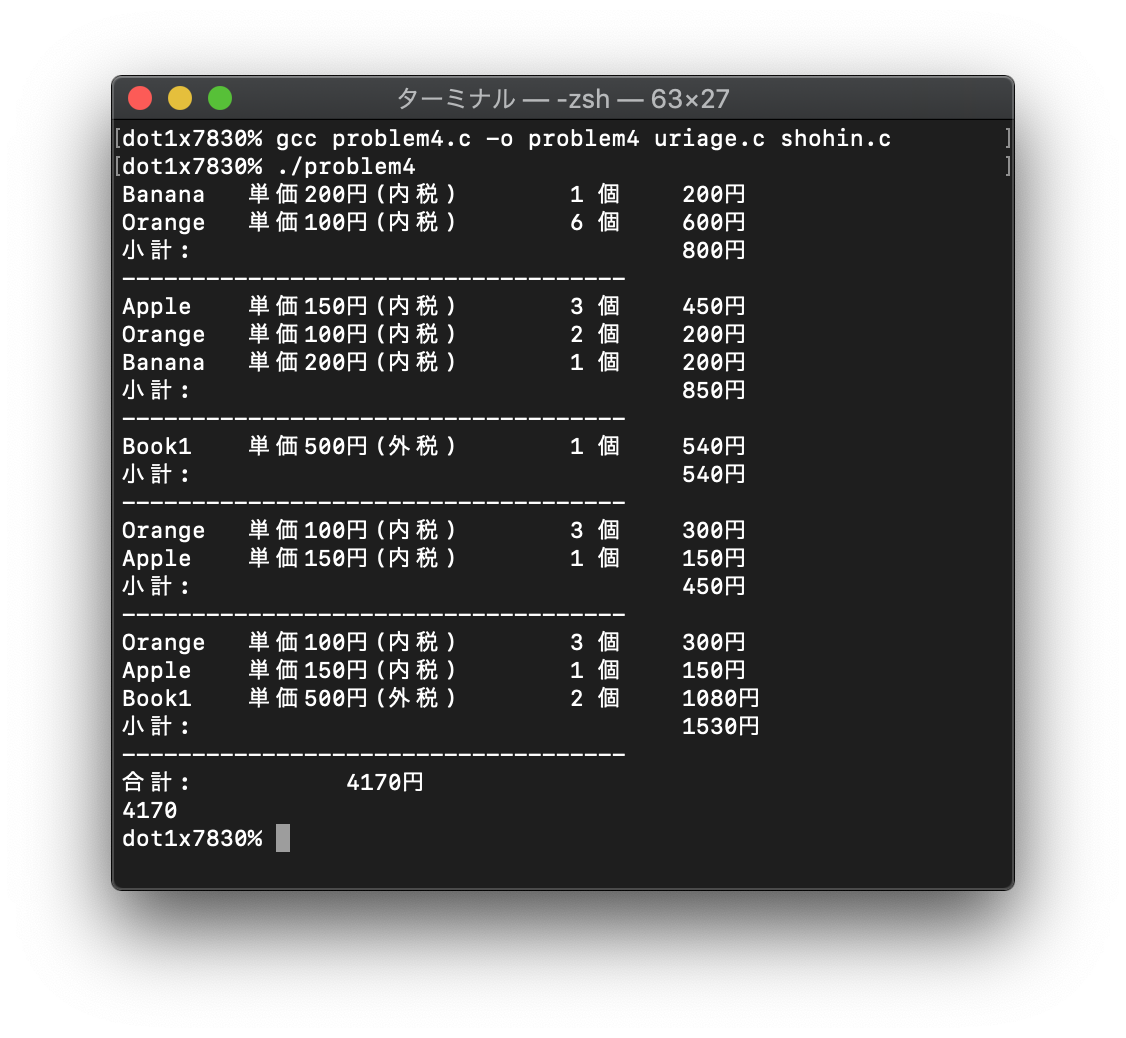
\includegraphics[width=0.8\textwidth]{problem1-4.png}
	\caption{問題1-4実行結果}
\end{figure}

\subsubsection{プログラムの解説}
[uriage.c]printUriageTrans関数は、URIAGE型のポインタのポインタ変数を引数とし、戻り値がintの関数である。
この関数にはmain()でuriage0[]~uriage4[]の先頭アドレスが格納されているURIAGE型ポインタ配列uriage[]が渡される。
for文では、main関数内のuriage配列に格納されている配列のアドレスをprintUriageArrayに渡し、戻り値をsub\_totalに格納する。totalには、total + sub\_totalの値を代入する。この処理をuriage配列の値がNULLになるまで繰り返す。
\pagebreak

\pagebreak

\subsection{考察}
今回の課題を解いてレポート書くにあたって構造体を宣言する方法や構造体のプロパティーを参照する方法について詳しく理解できた。そしてアロー演算子を使って構造体ポインターからプロパティーの値を参照する方法も理解できた。
また、ポインタとは変数のアドレスを格納する特殊な変数で、変数のアドレスをメモリのどこかに保存されていてポインタ変数も独自のアドレスを持つことができ、ポインタのポインタから、参照しているポインタがさらに参照している大元の変数へアクセスすることもできるということが分かった。そしてポインタを連鎖は無限にできるが、ポインタのポインタ以降の連鎖はプログラマ自身が参照先がどこなのかを把握しにくくなるため、通常は使用されないということが分かった。


\end{document}